\section{Parameterized Symbolic Dynamic Programming}
\label{sec:sdp}

Symbolic Dynamic Programming (SDP)~\parencite{Boutilier_IJCAI_2001} is the process of performing dynamic programming via symbolic manipulation. In the following sections we present a brief overview of SDP operations and how it can be adapted to solve Parameterized Hybrid MDPs.

\subsection{Symbolic Case Calculus}

SDP assumes that all functions can be represented in case statement form \parencite{Boutilier_IJCAI_2001} as follows:
{\footnotesize 
    \abovedisplayskip=5pt
    \belowdisplayskip=0pt
    \begin{align*}
        f = 
        \begin{cases}
            \phi_1: & f_1 \\ 
            \vdots & \vdots\\ 
            \phi_k: & f_k \\ 
        \end{cases}
    \end{align*}
}%

Here, {\footnotesize$ f_i $} are linear expressions over {\footnotesize$ \vec{x} $} and {\footnotesize$\phi_i$} are logical formulae defined over the state {\footnotesize$( \vec{d}, \vec{x})$} that can consist of arbitrary logical combinations of boolean variables and linear inequalities {\footnotesize$\left( \geq, >, <, \leq \right)$} over continuous variables. We assume that the set of conditions {\footnotesize$\left\lbrace \phi_1, \ldots, \phi_k \right\rbrace$} disjointly and exhaustively partition {\footnotesize$(\vec{d}, \vec{x})$} such that {\footnotesize$f$} is well-defined for all {\footnotesize$(\vec{d}, \vec{x})$}. In this paper we restrict the {\footnotesize$f_i$} to be either constant or linear functions of the state variables. Henceforth, we refer to functions with linear {\footnotesize$\phi_i$} and piecewise constant {\footnotesize$f_i$} as linear piecewise constant (LPWC), functions with linear {\footnotesize$\phi_i$} and piecewise linear {\footnotesize$f_i$} as linear piecewise linear (LPWL) and functions with nonlinear {\footnotesize$\phi_i$} and piecewise nonlinear {\footnotesize$f_i$} as nonlinear piecewise nonlinear (NPWN) functions.

Operations on case statements may be either unary or binary. All of the operations presented here are closed form for LPWC and LPWL functions. All operations except $\contmax_{y}$, presented below, is closed form for NPWN functions. We refer the reader to~\parencite{Sanner_UAI_2011,Zamani_AAAI_2012} for more thorough expositions of SDP for piecewise continuous functions.

Unary operations on a single case statement \emph{f}, such as scalar multiplication {\footnotesize$c \cdot f$} where {\footnotesize$ c \in \mathbb{R} $}, are applied to  each {\footnotesize$f_i \left(1 \leq i \leq k\right)$}. Binary operations such as addition, subtraction and multiplication are executed in two stages. Firstly, the cross-product of the logical partitions of each case statement is taken, producing paired partitions. Finally, the binary operation is applied to the resulting paired partitions. The ``cross-sum'' {\footnotesize$\oplus$} operation can be performed on two cases in the following manner:
{\footnotesize 
%    \abovedisplayskip=5pt
%    \belowdisplayskip=0pt
    \begin{center}
        \begin{tabular}{r c c c l}
            $\begin{cases}
            \phi_1: \hspace{-1mm} & \hspace{-1mm} f_1  \\ 
            \phi_2: \hspace{-1mm} & \hspace{-1mm} f_2  \\ 
            \end{cases}$
            $\oplus$
            &
            \hspace{-4mm}
            $\begin{cases}
            \psi_1: \hspace{-1mm} & \hspace{-1mm} g_1  \\ 
            \psi_2: \hspace{-1mm} & \hspace{-1mm} g_2  \\ 
            \end{cases}$
            &
            \hspace{-4mm} 
            $ = $
            &
            \hspace{-4mm}
            $\begin{cases}
            \phi_1 \wedge \psi_1: & f_1 + g_1 \\
            \phi_1 \wedge \psi_2: & f_1 + g_2 \\
            \phi_2 \wedge \psi_1: & f_2 + g_1 \\
            \phi_2 \wedge \psi_2: & f_2 + g_2  \\
            \end{cases}$
        \end{tabular}
    \end{center}
}%
%\vspace{-4em}

``cross-subtraction'' {\footnotesize$\ominus$} and ``cross-multiplication'' {\footnotesize$\otimes$} are defined in a similar manner but with the addition operator replaced by the subtraction and multiplication operators, respectively. Some partitions resulting from case operators may be inconsistent and are thus removed.

%Substitution into case statements is performed via a set {\footnotesize$\vartheta$} of variables and their substitutions e.g. {\footnotesize$\vartheta = \left\{ x'_1/(x_1 + x_2) \right\}$}, where the LHS of the / represents the substitution variable and the RHS of the / represents the expression that should be substituted in its place. {\footnotesize$\vartheta$} can be applied to both non-case functions {\footnotesize$f_i$} and case partitions {\footnotesize$\phi_i$} as {\footnotesize$f_i\vartheta$} and {\footnotesize$\phi_i\vartheta$}, respectively. Substitution into case statements can be written as:
%{\footnotesize 
%    \abovedisplayskip=5pt
%    \belowdisplayskip=0pt
%    \begin{align*}
%        f\vartheta = 
%        \begin{cases}
%            \phi_1\vartheta: & f_1\vartheta \\ 
%            \vdots & \vdots\\ 
%            \phi_k\vartheta: & f_k\vartheta \\ 
%        \end{cases}
%    \end{align*}
%}%
%
%Substitution is used when calculating integrals with respect to deterministic {\footnotesize$\delta$} transitions~\parencite{Sanner_UAI_2011}.

Maximisation over cases, known as $\casemax$, is defined as:
\vspace{-0.5em}
{\footnotesize 
    \abovedisplayskip=0pt
    \belowdisplayskip=0pt
    \begin{center}
        \begin{tabular}{r c c c l}
            \hspace{-7mm} 
            
            $\casemax \Bigg(
            \begin{cases}
            \phi_1: \hspace{-1mm} & \hspace{-1mm} f_1 \\ 
            \phi_2: \hspace{-1mm} & \hspace{-1mm} f_2 \\ 
            \end{cases}$
            $,$
            &
            \hspace{-4mm}
            $\begin{cases}
            \psi_1: \hspace{-1mm} & \hspace{-1mm} g_1 \\ 
            \psi_2: \hspace{-1mm} & \hspace{-1mm} g_2 \\ 
            \end{cases} \Bigg)$
            &
            \hspace{-4mm} 
            $ = $
            &
            \hspace{-4mm}
            $\begin{cases}
            \phi_1 \wedge \psi_1 \wedge f_1 > g_1    : & \hspace{-2mm} f_1 \\ 
            \phi_1 \wedge \psi_1 \wedge f_1 \leq g_1 : & \hspace{-2mm} g_1 \\ 
            \phi_1 \wedge \psi_2 \wedge f_1 > g_2    : & \hspace{-2mm} f_1 \\ 
            \phi_1 \wedge \psi_2 \wedge f_1 \leq g_2 : & \hspace{-2mm} g_2 \\ 
            \vdots & \vdots
            \end{cases}$
        \end{tabular}
    \end{center}
}%

$\casemax$ preserves the linearity of the constraints and the constant or linear nature of the {\footnotesize$f_i$} and {\footnotesize$g_i$}. If the {\footnotesize$f_i$} or {\footnotesize$g_i$} are quadratic then the expressions {\footnotesize$f_i > g_i$} or {\footnotesize$f_i \leq g_i$} will be at most univariate quadratic and any such constraint can be linearized into a combination of at most two linear inequalities by completing the square. 

A case statement can be maximized with respect to a continuous parameter {\footnotesize$y$} as {\footnotesize $ f_1(\vec{x}, y) = \contmax_{y}f_2(\vec{x}, y) $}. The continuous maximization operation is a complex case operation whose explanation is beyond the scope of this paper. We refer the reader to~\parencite{Zamani_AAAI_2012} for further details.

In principle, case statements can be used to represent all PHMDP components. In practice, case statements are implemented using a more compact representation known as Extended Algebraic Decision Diagrams (XADDs)~\parencite{Sanner_UAI_2011}, which also support efficient versions of all of the aforementioned operations. Figure~\ref{fig:xadd} shows how an XADD is used to represent a function {\footnotesize $f$} that is piecewise continuous, nonlinear and multimodal.

\begin{figure}[!htb]
%    \centering
    \begin{subfigure}[b]{0.20\textwidth}
        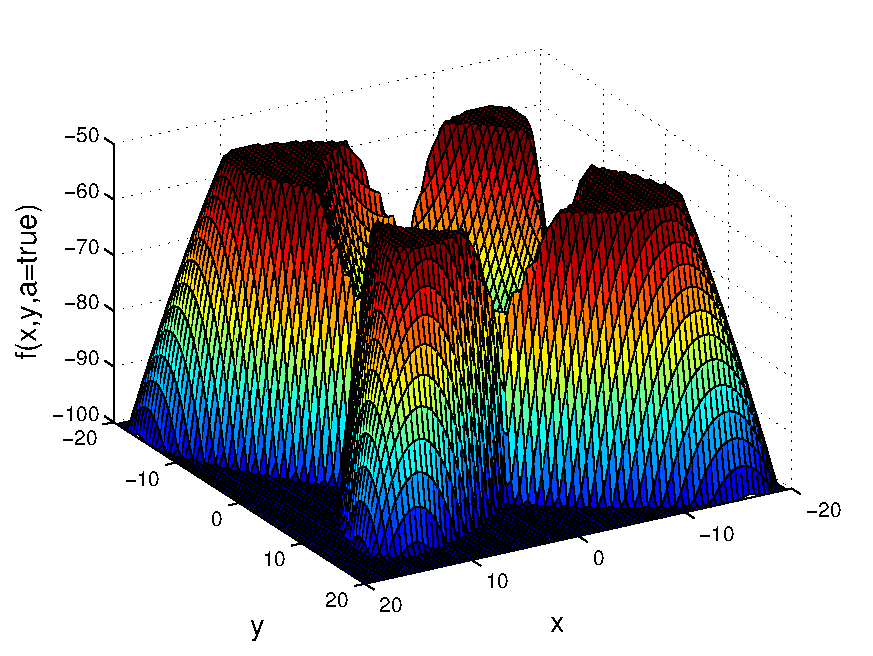
\includegraphics[width=1.0\linewidth]{images/quad2.pdf}
%        \caption{$f(x, y, a=\mathit{true})$}
    \end{subfigure}
            \hspace{-5mm}
    \begin{subfigure}[b]{0.24\textwidth}

        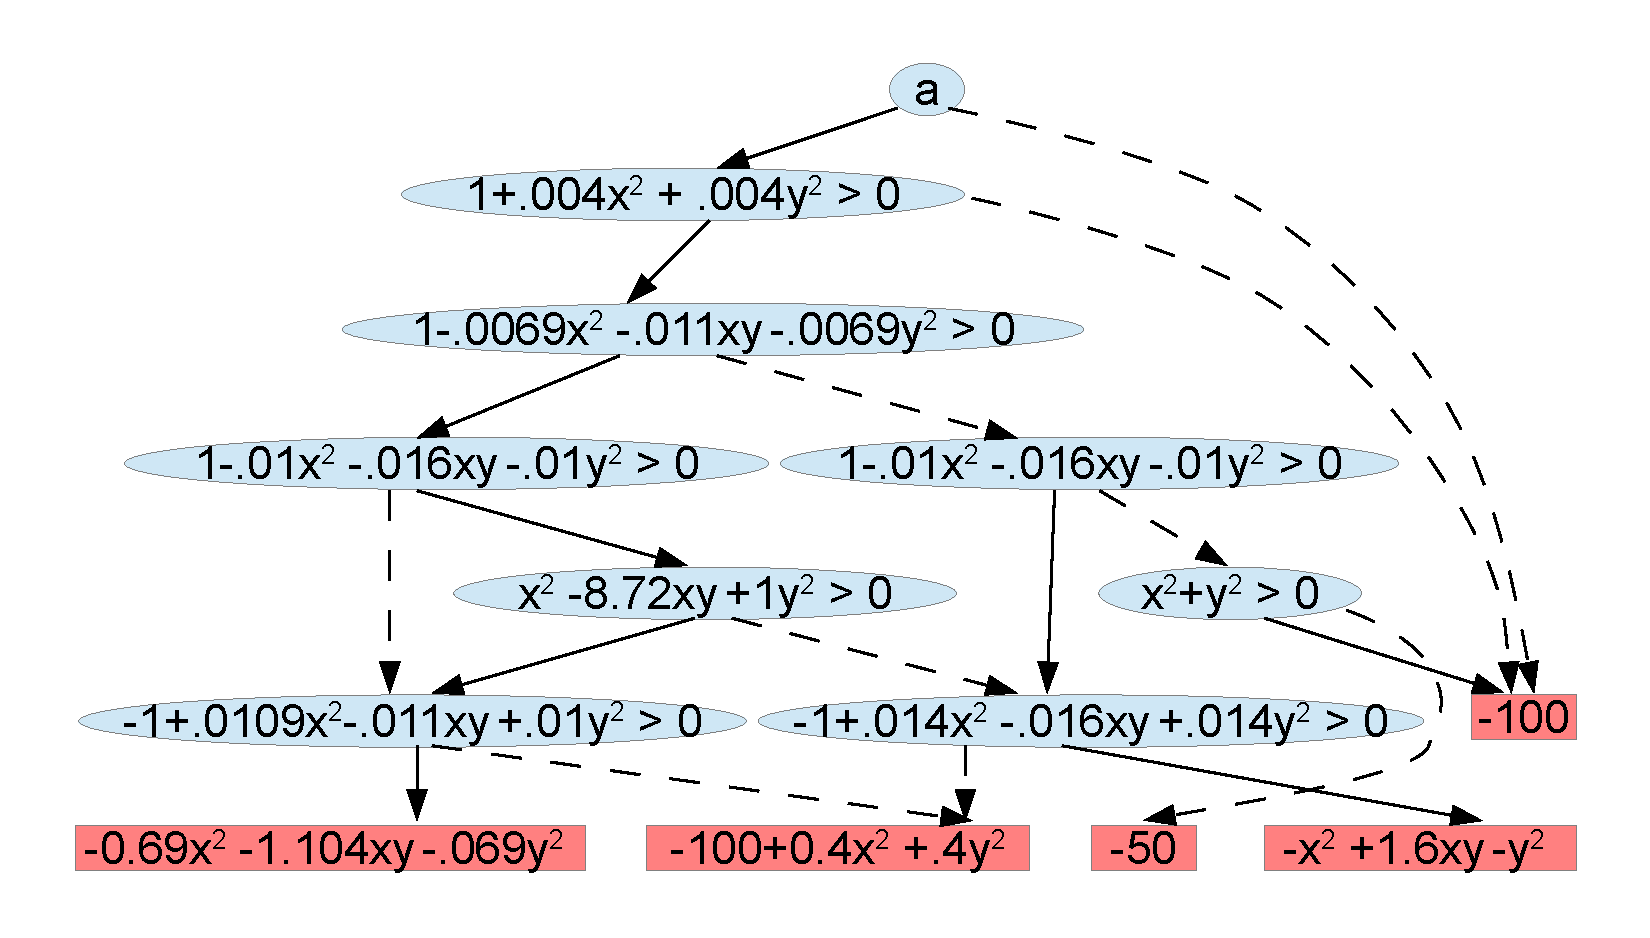
\includegraphics[width=1.3\linewidth, height=1.0\linewidth]{images/quad2_xadd5.pdf}
%        \caption{XADD representation}        
    \end{subfigure}    
    \caption{(left) A plot of a function $f(x, y, a=\mathit{true})$ for continuous variables $x$ and $y$ and boolean variable $a$; and (right) its XADD representation.}
    \label{fig:xadd}
\end{figure}

%\begin{figure*}[h!]
%    \vspace{-5mm}
%    \begin{center}
%        \begin{tabular}{ccc}
%            \hspace{-4mm} 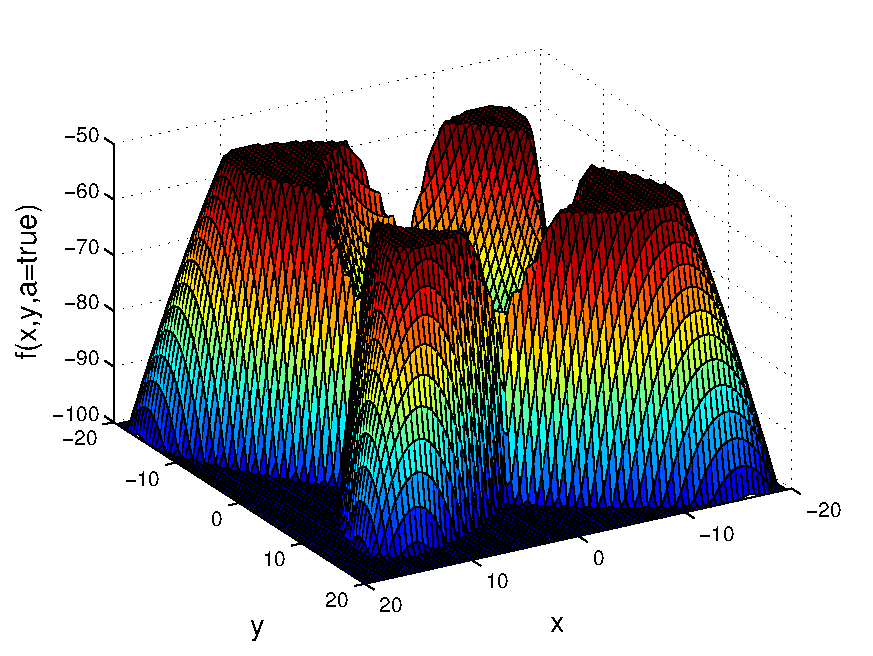
\includegraphics[width=0.35\textwidth]{images/quad2.pdf} & \hspace{-7.5mm} \includegraphics[width=0.30\textwidth]{images/quad2_contour2.pdf} & \hspace{-8mm} 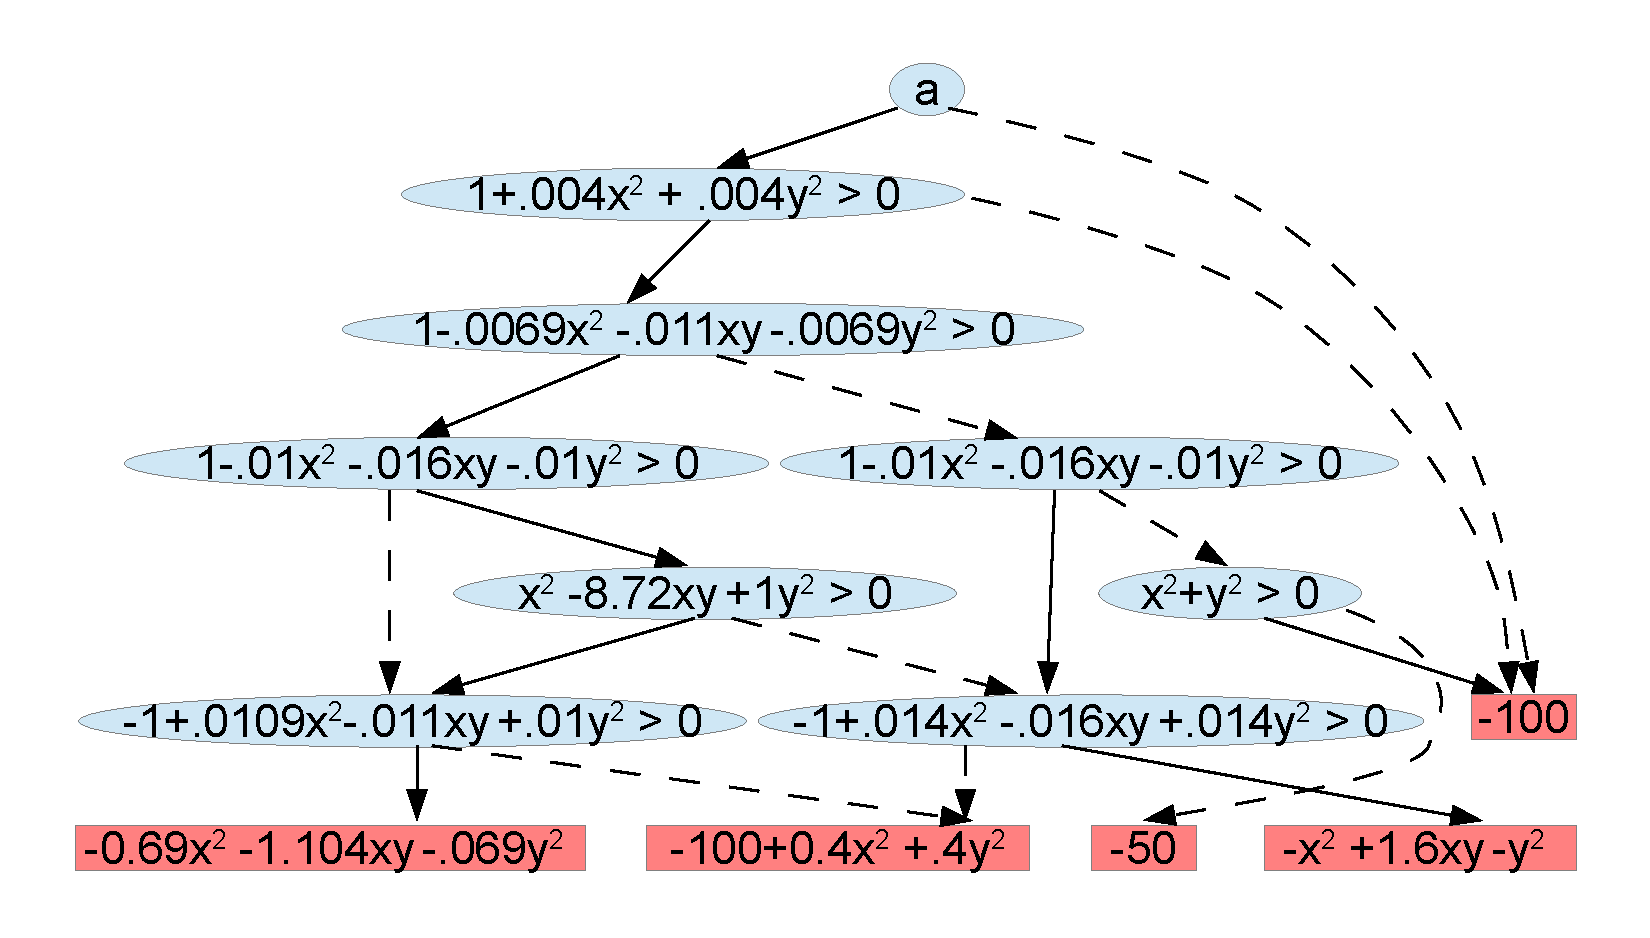
\includegraphics[width=0.40\textwidth]{images/quad2_xadd5.pdf}\\ 
%            %(a) & (b) & (c) \\
%            %\multicolumn{3}{c}{}
%        \end{tabular}
%    \end{center}
%    \vspace{-7mm}
%    \caption{\normalsize (left) A plot of a function $f(x, y, a=\mathit{true})$ for continuous variables $x$ and $y$ and boolean variable $a$; (middle) a
%        contour plot of $f(x,y,a=\mathit{true})$ showing sharp piecewise boundaries; and (right) an XADD representing $f(x,y,a)$. $f$ is \emph{piecewise continuous}, \emph{nonlinear}, and \emph{multimodal}; it has a compact symbolic XADD representation as indicated by its highly recurrent directed acyclic graph (DAG) structure.  }
%    \label{fig:xadd}
%    \vspace{-2mm}
%\end{figure*}

\subsection{SDP for Parameterized Hybrid MDPs}

To calculate the exact solution to PHMDPs we begin by replacing all functions and operations in Equations~\eqref{eq:vi_qfunc} and~\eqref{eq:vi_vfunc} by their case statement equivalents. That is, we exchange operations such as {\footnotesize$+$}, {\footnotesize$\times$} and {\footnotesize$\max$}, by their symbolic equivalents, {\footnotesize$\oplus$}, {\footnotesize$\otimes$} and $\casemax$, respectively, and express {\footnotesize $\Reward(\vec{d}, \vec{x}, a; \vec{\theta})$},  {\footnotesize $\ProbArg{\vec{d}', \vec{x}' | \vec{d}, \vec{x}, a, \vec{\theta}}$}, {\footnotesize $V^0(\vec{d}, \vec{x}; \vec{\theta})$} as case statements. The optimal solution to PHMDPs can now be described by the following recursive SDP equations:
{\footnotesize 
    \abovedisplayskip=0pt
    \belowdisplayskip=0pt
    \begin{align}
        Q^{h} \left( \vec{d}, \vec{x}, a; \vec{\theta} \right) = \Reward \left( \vec{d}, \vec{x}, a; \vec{\theta} \right) \oplus \gamma \, \cdot &  \nonumber \\ 
        \bigoplus_{\vec{d}'} \int_{\vec{x}'} \ProbArg{ \left. \vec{d}', \vec{x}' \middle| \vec{d}, \vec{x}, a; \vec{\theta} \right.} \otimes V^{h-1} \left( \vec{d}', \vec{x}'; \vec{\theta} \right) & \, d\vec{x}'  \label{eq:vi_sdp_qfunc} \\
        V^{h}\left( \vec{d}, \vec{x}; \vec{\theta} \right) = \casemax_{a \in A} \left\{ Q^{h} \left( \vec{d}, \vec{x}, a; \vec{\theta} \right) \right\} & \label{eq:vi_sdp_vfunc}
    \end{align}
}%

{\footnotesize $\ProbArg{\left. \vec{d}', \vec{x}' \middle| \vec{d}, \vec{x}, a; \vec{\theta} \right.}$ } is specified in Equation~\eqref{eq:hmdp_tfunc}. We note that all parameters {\footnotesize $\theta_i$} that are free variables 
are encoded as {\footnotesize $\delta\left[\left(\theta_i' - \theta_i\right)\right]$}, indicating that they are stationary and hence do not change during the backup operation. Continuous state parameters {\footnotesize $ \vec{x} $} are handled in a similar fashion. All operations including action maximization will automatically condition the value on these parameters, yielding the parameterized value function in Equation~\eqref{eq:vi_sdp_vfunc}.

In the case of discrete {\footnotesize \Action} it can be proved that all of the SDP operations used in Equations~\eqref{eq:vi_sdp_qfunc} and~\eqref{eq:vi_sdp_vfunc} are closed form for NPWN functions~\parencite{Sanner_UAI_2011}. In the case of continuous {\footnotesize \Action} all of the operations are closed form for only LPWC or LPWL functions~\parencite{Zamani_AAAI_2012}.

%It can be proved that all of the SDP operations used in Equations~\eqref{eq:vi_qfunc} and~\eqref{eq:vi_vfunc} are closed form for LPWC or LPWL functions~\parencite{Sanner_UAI_2011,Zamani_AAAI_2012}. Given a LPWL {\footnotesize $V^{0}(\vec{d}, \vec{x}; \vec{\theta})$} and that SDP operations are closed form, the resulting {\footnotesize $V^{1}(\vec{d}, \vec{x}; \vec{\theta})$} is also LPWL. Therefore, by induction is {\footnotesize $V^{h+1}(\vec{d}, \vec{x}; \vec{\theta})$} LPWL for all horizons {\footnotesize $ \Horizon $}. 

\subsubsection{Inverse Learning for Multi-objective PHMDPs}

The inverse learning problem for multi-objective MDPs, whereby observed behavior is used to infer multi-objective weights that explain the observed behavior, has many possible formulations. One possible formulation is to constrain the Q-values corresponding to the observed behavior and maximize the weight {\footnotesize $ w $} that most explains the observed behavior: 
\begin{align}
    \max_w Q^{h} \left(w, \vec{d}, x, a_1; \vec{\theta}^d \right) \ominus Q^{h} \left(w, \vec{d}, x, a_2; \vec{\theta}^d \right)
\end{align}
where {\footnotesize $ x $} can either be fixed or a region specified in the constraints. The PHMDP framework permits any variant of the inverse learning problem for multi-objective MDPs.

PHMDPs with multi-objective {\footnotesize $\Reward$} and linear scalarization functions can be solved exactly and in closed-form by restricting the {\footnotesize $\Reward$} to LPWC functions and {\footnotesize $\Transition$} to LPWL functions. Given a LPWL {\footnotesize $V^{0}(\vec{d}, \vec{x}; \vec{\theta})$} and that SDP operations are closed form, the resulting {\footnotesize $V^{1}(\vec{d}, \vec{x}; \vec{\theta})$} is also LPWL. Therefore, by induction {\footnotesize $V^{h+1}(\vec{d}, \vec{x}; \vec{\theta})$} is LPWL for all horizons {\footnotesize $ h \in \Horizon $}. Multi-objective PHMDPs with a nonlinear scalarization function and NPWN {\footnotesize $\Reward$} and {\footnotesize $\Transition$} functions lead NPWN solutions, which are exact and closed-form~\parencite{Sanner_UAI_2011}.

\subsubsection{Sensitivity Analysis for PHMDPs}

%Sensitivity analysis for PHMDPs can be conducted exactly and in closed-form by firstly imposing the same restrictions on the {\footnotesize $\Reward$} and {\footnotesize $\Transition$} as the previous section and then differentiating the resulting value function with respect to the parameter {\footnotesize $\vec{\theta}$} i.e. {\footnotesize $\bigtriangledown_{\vec{\theta}} V^{h}\left(\vec{d}, \vec{x}; \vec{\theta}\right)$ }.

Sensitivity analysis for PHMDPs can be analysed exactly and in closed-form via SDP by first calculating Equation~\eqref{eq:vi_sdp_vfunc} and then taking symbolic derivatives, up to any order, with respect to the parameter {\footnotesize $\vec{\theta}^{d}$}.

% i.e. {\footnotesize $\bigtriangledown_{\vec{\theta}^{d}} V^{h}\left(\vec{d}, \vec{x}; \vec{\theta}^{d}\right)$}.

\subsubsection{Nonlinear Parameterized Policy Optimization Methods for PHMDPs}

Parameterized policies {\footnotesize $ \pi(\vec{\theta}^{d}) $}, where {\footnotesize $\vec{\theta}^{d}$} may be nonlinear, for PHMDPs can be analyzed exactly and in closed-form via SDP by substituting {\footnotesize $ \pi(\vec{\theta}^{d}) $} in for {\footnotesize  $ a $} in Equation~\eqref{eq:vi_sdp_qfunc}. This precludes the need for action maximization in Equation~\eqref{eq:vi_sdp_vfunc}. Because this function is parametric, it is possible to take symbolic derivatives up to any order i.e. {\footnotesize $\bigtriangledown_{\vec{\theta}^{d}} Q^{h}(\vec{d}, \vec{x}, a; \vec{\theta}^{d})$ } and apply non-convex optimization tools, such as dReal or dOp~\parencite{Gao2013}, that exploit parametric knowledge of the function. Symbolic derivatives avoid the stochasticity issues associated with traditional policy gradient methods.

In the next section we demonstrate how PHMDPs can be combined with SDP and state-of-the-art nonlinear optimization techniques to solve hard nonlinear sequential decision problems that were previously impossible.